\documentclass{article}
\usepackage[top=1in, bottom=1in, left=1in, right=1in]{geometry}
% \usepackage{fullpage, fancyhdr}
\usepackage{fullpage}
\usepackage{float}
\usepackage{mathtools}
\usepackage{xfrac}
\usepackage{graphicx}
\usepackage{caption}
\usepackage{subcaption}
\usepackage{portland}
%\usepackage{setspace}
\setlength{\topmargin}{0.0in}
\setlength{\headheight}{0.5in}
\setlength{\headsep}{0in}
\setlength{\footskip}{9pt}
\usepackage{listings}
\usepackage{color}

\usepackage{multicol}

\renewcommand{\arraystretch}{1.5}

\newcommand{\Lagr}{\mathcal{L}}

% For circuitikz
\usepackage[american,arrowmos]{circuitikz}
\usepackage{tikz}
\usetikzlibrary{calc}
\usepackage{pgfplots}
\usepackage{amsfonts}
\usetikzlibrary{shapes,arrows}

% \pagestyle{fancyplain}
\pagestyle{myheadings}
\voffset=-0.50in
\topmargin=0.00in 
\headsep=0.25in 
\evensidemargin=0in 
\oddsidemargin=0in 
\textwidth=6.6in 
\textheight=10.0in 

\renewcommand{\topfraction}{0.9}	% max fraction of floats at top
\renewcommand{\bottomfraction}{0.8}	% max fraction of floats at bottom
%   Parameters for TEXT pages (not float pages):
\setcounter{topnumber}{2}
\setcounter{bottomnumber}{2}
\setcounter{totalnumber}{4}     % 2 may work better
\setcounter{dbltopnumber}{2}    % for 2-column pages
\renewcommand{\dbltopfraction}{0.9}	% fit big float above 2-col. text
\renewcommand{\textfraction}{0.07}	% allow minimal text w. figs
%   Parameters for FLOAT pages (not text pages):
\renewcommand{\floatpagefraction}{0.7}	% require fuller float pages
% N.B.: floatpagefraction MUST be less than topfraction !!
\renewcommand{\dblfloatpagefraction}{0.7}	% require fuller float pages
% remember to use [htp] or [htpb] for placement

\title{Assignment \# 8: Hearing Loss, Accelerometers, and Control Systems}
\date{4/08/2013}
\author{Brian Arnberg}

\markright{Brian Arnberg\hfill ELEC 6760 - Solid State Sensors\hfill}     
\setlength{\parindent}{0pt}


\begin{document}\label{start}

% \begin{titlepage}
% 	\maketitle
% 	\thispagestyle{empty}
% \end{titlepage}


\section*{ Homework Assignment \#8 - Due Mon. 4/08/13 }
\renewcommand{\labelenumi}{\arabic{enumi})}
\begin{multicols}{2}
\begin{enumerate}
%--------------------------------------------------------------%
%---- Problem 1 -----------------------------------------------%
\item\label{p1}
 You decide to attend a rock concert without earplugs. You sit where the sound
     power level is 109 dB. How long until you have permanent hearing loss?

		\begin{tabular}{ l }
			$109dB \rightarrow 1.875\text{min}$,\\
			per ``Decibel Exposure Time Guidelines''
		\end{tabular}
%--------------------------------------------------------------%
%---- Problem 2 -----------------------------------------------%
\item\label{p2}
At the rock concert in (\ref{p1}), you decide to sit in the back where the sound power
     level is only 103 dB. How long until you have permanent hearing loss?
	
		\begin{tabular}{ l }
			$103dB \rightarrow 7.5\text{min}$,\\
			per ``Decibel Exposure Time Guidelines''
		\end{tabular}
  
%--------------------------------------------------------------%
%---- Problem 3 -----------------------------------------------%
\item\label{p3}
 A doubled clamped spring style accelerometer consists of a Si proof mass (500$\mu$m
     thick and 1mm by 1mm) and a suspension system (2 rectangular beams, one on
     one side and one on the other side of the PM, 100$\mu$m long, 10$\mu$m wide and 5$\mu$m
     thick). For a Young's modulus of 190GPA and a density of 2.3$g/cm^3$, what is the
     sensitivity of the accelerometer?

		\begin{tabular}{ l }
			$S = m/K_s \colon m = \rho * v \colon K_s = \frac{N_{LEG}}{N_{ZIG}}\frac{E\times w \times t^3}{L^3}$\\
			$m = 2.3 g/cm^3 \times \frac{(100^3)cm^3 \times kg}{1000g\times m^3} \times (500\mu m)(1mm)^2$\\
			$m = 1.15 \times 10^{-6} kg$\\
			$K_s = \frac{2}{1} \times \frac{190 \times 10^9 (10\times10^{-6})(5\times10^{-6})^3}{(100\times10^{-6})^3}$\\
			$K_s = 475N/m$\\
			$S = m/K_s = \frac{1.15\times10^{-6}}{475N/m}$\\
			$S = 2.42 \times 10^{-9} s^2$
		\end{tabular}
%--------------------------------------------------------------%
%---- Problem 4 -----------------------------------------------%
\item\label{p4}
For an accelerometer with a natural frequency of 1000Hz, what is the proof mass /
     frame relative displacement for a 10 G acceleration \\(1G = 9.8 $m/s^2$)?
	
		\begin{tabular}{ l }
			$d = a \times S \colon \omega_n = 2 \pi 1000 \colon a = 10 \times 9.8 m/s^2$\\

			$S = \frac{1}{\omega_n^2} = \frac{1}{(2 \pi 1000)^2} = 25.33\times 10^{-9} s^2$\\
			$d = a\times S = 10 \times 9.8 \times 25.33 \times 10^{-9}$\\
			$d = 2.48 \mu m$
		\end{tabular}
  
%--------------------------------------------------------------%
%---- Problem 5 -----------------------------------------------%
\item\label{p5}
What is the natural frequency (in Hz) for an accelerometer where a 10 G
     acceleration (1G = $9.8 m/s^2$) results in a proof mass / frame relative displacement
     of 10$\mu m$?

		\begin{tabular}{ l }
			$d = 10\mu m \colon a = 10\times 9.8 m/s^2$\\
			$S = d/a = \frac{10\mu m}{10*9.8} =  102.04 \times 10^{-9} s^2$\\
			$S = (\omega_n^2)^{-1} \rightarrow \omega_n = \sqrt{1/S}$\\
			$\omega_n = \sqrt{1/(102.04 \times 10^{-9} s^2)} = 3.13 k rad/s$\\
			$f_n = \omega_n /(2\pi) = 498 Hz$
		\end{tabular}

%--------------------------------------------------------------%
%---- Problem 6 -----------------------------------------------%
\item\label{p6}
For a(t) = 2u(t), what is Vout(t)? (See figure below)
	
\begin{tabular}{ l }
	$E(s) = A(s) - V_{out}(s) \colon V_{out}(s) = E(s)(1/s)$\\
	$V_{out} = (A(s) - V_{out}(s))(1/s) \rightarrow V_{out}(s) = \frac{A(s)}{s+1}$\\
	$A(s) = 2*(1/s) \rightarrow V_{out}(s) = \frac{2}{s^2 + s}$\\
	$V_{out}(s) = \frac{2}{s} - \frac{2}{s+1}$\\
	$V_{out}(t) = \Lagr^{-1}[\frac{2}{s} - \frac{2}{s+1}]$\\
	$V_{out}(t) = 2(1) - 2(e^{-t}) = 2(1-e^{-t})$

\end{tabular}

%----- End Enumerate ------------------------------------------%
\end{enumerate}
%----- End Columns --------------------------------------------%
\end{multicols}

%--------------------------------------------------------------%
%---- Bottom of the page Figure -------------------------------%
\begin{figure}[h]
	\centering
	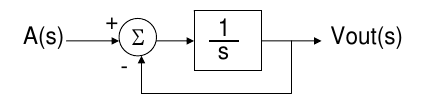
\includegraphics[keepaspectratio,width=0.50\textwidth]{control}
\end{figure}

\label{end}\end{document}


